% Architecture of the kimauve shop and buyer in Round 3 (week-08 midterm). Build: pdflatex architecture.tex
% Each box: name, who runs it (code or which model), one or two lines of what it does. Details are in REPORT.md.
\documentclass[border=8pt]{standalone}
\usepackage[T1]{fontenc}
\usepackage{lmodern}
\usepackage{tikz}
\usetikzlibrary{positioning,fit,backgrounds,arrows.meta,calc}

\definecolor{code}{HTML}{2F6DB5}
\definecolor{model}{HTML}{B5462F}
\definecolor{mem}{HTML}{5E7D2F}
\definecolor{kit}{HTML}{7A7A7A}
\definecolor{ours}{HTML}{FFF4D6}

\tikzset{
  box/.style={draw, rounded corners=2pt, align=left, font=\footnotesize, inner sep=4pt,
              text width=4.0cm, minimum height=1.25cm, fill=white,
              execute at begin node={\hyphenpenalty=10000 \exhyphenpenalty=10000 }},
  codebox/.style={box, draw=code, line width=0.9pt},
  modelbox/.style={box, draw=model, line width=0.9pt, fill=model!6},
  membox/.style={draw=mem, rounded corners=2pt, fill=mem!7, font=\scriptsize, align=left,
                 text width=3.7cm, inner sep=3pt, minimum height=0.62cm},
  kitbox/.style={draw=kit, dashed, rounded corners=2pt, fill=kit!6, font=\footnotesize, align=center, inner sep=4pt},
  flow/.style={-{Latex[length=2mm]}, line width=0.6pt},
  feed/.style={-{Latex[length=2mm]}, line width=0.7pt, mem!75!black},
  fix/.style={-{Latex[length=2mm]}, line width=0.9pt, model, dashed},
  lbl/.style={font=\scriptsize\itshape, fill=white, inner sep=1pt},
  band/.style={font=\scriptsize\bfseries, text=black!55, anchor=east},
  group/.style={draw=black!25, rounded corners=4pt, inner sep=7pt, fill=ours},
}
% name on the left, runner on the right, then the description
\newcommand{\hd}[3]{\textbf{#1}\hfill\textcolor{#2}{#3}\\[2pt]}

\begin{document}
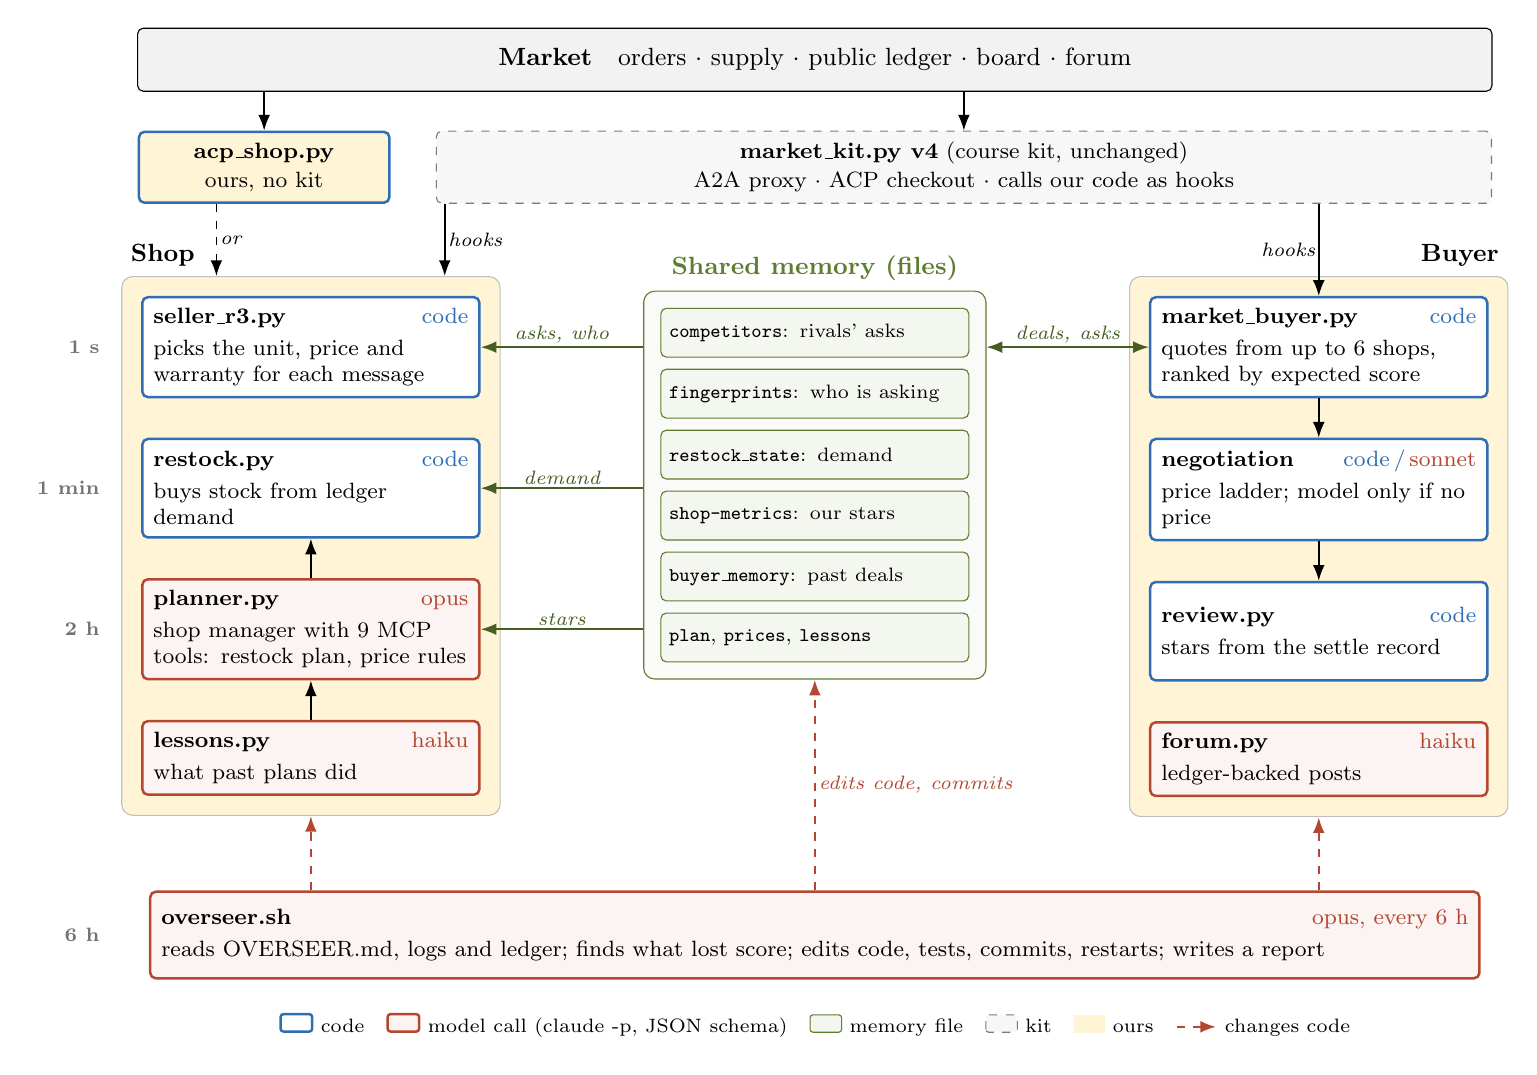
\begin{tikzpicture}

% ---------------- market and kit ----------------
\node[draw, rounded corners=2pt, fill=black!5, minimum width=17.2cm, minimum height=0.8cm, font=\small] (market) at (0,0)
  {\textbf{Market}\quad orders $\cdot$ supply $\cdot$ public ledger $\cdot$ board $\cdot$ forum};

\node[kitbox, minimum width=13.4cm, minimum height=0.9cm, anchor=north east] (kit) at (8.6,-0.9)
  {\textbf{market\_kit.py v4} (course kit, unchanged)\\[1pt]
   A2A proxy $\cdot$ ACP checkout $\cdot$ calls our code as hooks};
\node[box, codebox, fill=ours, text width=2.9cm, minimum height=0.9cm, align=center, anchor=north west] (acp) at (-8.6,-0.9)
  {\textbf{acp\_shop.py}\\[1pt] ours, no kit};

% ---------------- shop column ----------------
\node[codebox, anchor=north] (seller) at (-6.4,-3.0)
  {\hd{seller\_r3.py}{code}{code}picks the unit, price and warranty for each message};
\node[codebox, below=0.5cm of seller] (restock)
  {\hd{restock.py}{code}{code}buys stock from ledger demand};
\node[modelbox, below=0.5cm of restock] (planner)
  {\hd{planner.py}{model}{opus}shop manager with 9 MCP tools: restock plan, price rules};
\node[modelbox, below=0.5cm of planner, minimum height=0.8cm] (lessons)
  {\hd{lessons.py}{model}{haiku}what past plans did};

% ---------------- buyer column ----------------
\node[codebox, anchor=north] (mbuyer) at (6.4,-3.0)
  {\hd{market\_buyer.py}{code}{code}quotes from up to 6 shops, ranked by expected score};
\node[codebox, below=0.5cm of mbuyer] (nego)
  {\hd{negotiation}{code}{code\,/\,\textcolor{model}{sonnet}}price ladder; model only if no price};
\node[codebox, below=0.5cm of nego] (review)
  {\hd{review.py}{code}{code}stars from the settle record};
\node[modelbox, below=0.5cm of review, minimum height=0.8cm] (forum)
  {\hd{forum.py}{model}{haiku}ledger-backed posts};

% ---------------- shared memory ----------------
\node[membox, anchor=north] (m1) at (0,-3.15) {\texttt{competitors}: rivals' asks};
\node[membox, below=0.14cm of m1] (m2) {\texttt{fingerprints}: who is asking};
\node[membox, below=0.14cm of m2] (m3) {\texttt{restock\_state}: demand};
\node[membox, below=0.14cm of m3] (m4) {\texttt{shop-metrics}: our stars};
\node[membox, below=0.14cm of m4] (m5) {\texttt{buyer\_memory}: past deals};
\node[membox, below=0.14cm of m5] (m6) {\texttt{plan}, \texttt{prices}, \texttt{lessons}};
\begin{scope}[on background layer]
  \node[draw=mem, rounded corners=4pt, fill=mem!3, inner sep=6pt, fit=(m1)(m6),
        label={[font=\small\bfseries, text=mem]above:Shared memory (files)}] (memg) {};
  \node[group, fit=(seller)(lessons), label={[font=\small\bfseries, anchor=south west]north west:Shop}] (shopg) {};
  \node[group, fit=(mbuyer)(forum), label={[font=\small\bfseries, anchor=south east]north east:Buyer}] (buyg) {};
\end{scope}

% ---------------- overseer ----------------
\node[modelbox, text width=16.6cm, minimum height=1.1cm, anchor=north] (over) at ($(0,0 |- lessons.south)+(0,-1.2)$)
  {\hd{overseer.sh}{model}{opus, every 6 h}reads OVERSEER.md, logs and ledger; finds what lost score; edits code, tests, commits, restarts; writes a report};

% ---------------- time bands ----------------
\node[band] at ($(shopg.west |- seller)+(-0.15,0)$) {1 s};
\node[band] at ($(shopg.west |- restock)+(-0.15,0)$) {1 min};
\node[band] at ($(shopg.west |- planner)+(-0.15,0)$) {2 h};
\node[band] at ($(shopg.west |- over)+(-0.15,0)$) {6 h};

% ---------------- control flow ----------------
\draw[flow] (market.south -| kit.north) -- (kit.north);
\draw[flow] (market.south -| acp.north) -- (acp.north);
\draw[flow] (kit.south -| mbuyer.north) -- node[lbl, left]{hooks} (mbuyer.north);
\draw[flow] (kit.south -| -4.7,0) -- node[lbl, right]{hooks} (-4.7,0 |- shopg.north);
\draw[flow, dashed] (acp.south -| -7.6,0) -- node[lbl, right]{or} (-7.6,0 |- shopg.north);
\draw[flow] (mbuyer) -- (nego);
\draw[flow] (nego) -- (review);
\draw[flow] (lessons) -- (planner);
\draw[flow] (planner) -- (restock);

% ---------------- memory feeds (horizontal) ----------------
\draw[feed] (memg.west |- seller) -- node[lbl, above]{asks, who} (seller.east);
\draw[feed] (memg.west |- restock) -- node[lbl, above]{demand} (restock.east);
\draw[feed] (memg.west |- planner) -- node[lbl, above]{stars} (planner.east);
\draw[feed, {Latex[length=2mm]}-{Latex[length=2mm]}] (mbuyer.west) -- node[lbl, above]{deals, asks} (memg.east |- mbuyer.west);

% ---------------- overseer edits code ----------------
\draw[fix] (over.north -| shopg.south) -- (shopg.south);
\draw[fix] (over.north -| buyg.south) -- (buyg.south);
\draw[fix] (over.north -| memg.south) -- node[lbl, right]{edits code, commits} (memg.south);

% ---------------- legend ----------------
\node[below=0.3cm of over, font=\scriptsize] {
  \tikz{\draw[code, line width=0.9pt, rounded corners=1pt] (0,0) rectangle (0.4,0.22);} code\quad
  \tikz{\draw[model, line width=0.9pt, fill=model!6, rounded corners=1pt] (0,0) rectangle (0.4,0.22);} model call (claude -p, JSON schema)\quad
  \tikz{\draw[mem, fill=mem!7, rounded corners=1pt] (0,0) rectangle (0.4,0.22);} memory file\quad
  \tikz{\draw[kit, dashed, fill=kit!6, rounded corners=1pt] (0,0) rectangle (0.4,0.22);} kit\quad
  \tikz{\fill[ours] (0,0) rectangle (0.4,0.22);} ours\quad
  \tikz{\draw[fix] (0,0.11) -- (0.5,0.11);} changes code};

\end{tikzpicture}
\end{document}
